\listfiles
\documentclass[review, 12pt]{elsarticle}

\usepackage{color}
\usepackage{subfig}
\usepackage{gensymb}
\usepackage{graphics}
\usepackage{graphicx}

\usepackage[colorlinks=true]{hyperref}
\usepackage{lineno}
\modulolinenumbers[5]

\journal{Journal of \LaTeX\ Templates}

%%%%%%%%%%%%%%%%%%%%%%%
%% Elsevier bibliography styles
%%%%%%%%%%%%%%%%%%%%%%%
%% To change the style, put a % in front of the second line of the current style and
%% remove the % from the second line of the style you would like to use.
%%%%%%%%%%%%%%%%%%%%%%%

% Numbered
% \bibliographystyle{model1-num-names}

%% Numbered without titles
% \bibliographystyle{model1a-num-names}

%% Harvard
% \bibliographystyle{model2-names}\biboptions{authoryear}

%% Vancouver numbered
% \usepackage{numcompress}\bibliographystyle{model3-num-names}

%% Vancouver name/year
% \usepackage{numcompress}\bibliographystyle{model4-names}\biboptions{authoryear}

%% APA style
\bibliographystyle{model5-names}\biboptions{authoryear}

\hypersetup{
  urlcolor     = blue, %Colour for external hyperlinks
  linkcolor    = blue, %Colour of internal links
  citecolor   = red, % Colour of citations
  %hidelinks
}

% Dossier des figures 
%\graphicspath{{figs/}{../figs/}}
\graphicspath{ {figs/} }

% Liste des extensions de figures (pour pdflatex)
\DeclareGraphicsExtensions{.pdf,.png,.jpg,.tiff}

%% AMA style
% \usepackage{numcompress}\bibliographystyle{model6-num-names}

%% `Elsevier LaTeX' style, distributed in TeX Live 2019
%\bibliographystyle{elsarticle-num}
% \usepackage{numcompress}\bibliographystyle{elsarticle-num-names}
% \bibliographystyle{elsarticle-harv}\biboptions{authoryear}
%%%%%%%%%%%%%%%%%%%%%%%


\newcommand{\warn}[1]{\textbf{\color{red}{#1}}}
\newcommand\nino{El Ni\~no}
\newcommand\nina{La Ni\~na}
\newcommand\ap{APECOSM}
\newcommand\hov{Hovm\"oller}
\newcommand\ppar{photosynthetically active radiation}
\newcommand\omz{oxygen minimum zone}
\newcommand\phy{nano-phytoplankton}
\newcommand\Phy{Nano-phytoplankton}
\newcommand{\phyd}{diatoms}
\newcommand{\Phyd}{Diatoms}
\newcommand\zoo{micro-zooplankton}
\newcommand\Zoo{Micro-zooplankton}
\newcommand{\zood}{meso-zooplankton}
\newcommand{\Zood}{Meso-zooplankton}
\newcommand{\goc}{big organic carbon}
\newcommand{\Goc}{Big organic carbon}
\newcommand{\cpn}{Central Pacific \nino}
\newcommand{\epn}{Eastern Pacific \nino}
\newcommand{\sst}{sea-surface temperature}
\newcommand{\enso}{El Ni\~no/Southern Oscillation}
\newcommand{\degN}{\degree N}
\newcommand{\degS}{\degree S}
\newcommand{\degE}{\degree E}
\newcommand{\degW}{\degree W}



\begin{document}


\begin{frontmatter}

\title{Impacts of ENSO variability on the simulated epipelagic fish biomass of the Tropical Pacific.}
%\tnotetext[mytitlenote]{Fully documented templates are available in the elsarticle package on \href{http://www.ctan.org/tex-archive/macros/latex/contrib/elsarticle}{CTAN}.}

%% Group authors per affiliation:
\author[mymainaddress]{Nicolas Barrier\corref{mycorrespondingauthor}}
%\address{Radarweg 29, Amsterdam}
\fntext[myfootnote]{MARBEC, Univ. Montpellier, CNRS, Ifremer, IRD, Sète, France}

\author[mymainaddress]{Olivier Maury}
\author[mymainaddress]{Matthieu Lengaigne}
\author[renaud]{Renaud Person}
\author[chris]{Christian Eth\'{e}}

\cortext[mycorrespondingauthor]{Corresponding author}

%% or include affiliations in footnotes:
%\author[mymainaddress,mysecondaryaddress]{Elsevier Inc}
%\ead[url]{www.elsevier.com}
%\author[mysecondaryaddress]{Global Customer Service\corref{mycorrespondingauthor}}
%\ead{support@elsevier.com}
\address[mymainaddress]{MARBEC, Univ. Montpellier, CNRS, Ifremer, IRD, Sète, France}
\address[renaud]{LOCEAN, IRD}
\address[chris]{IPSL, CNRS}

\begin{abstract}

\end{abstract}

\begin{keyword}
fish \sep biomass \sep ENSO \sep \nino \sep \nina \sep modelling
\end{keyword}

\end{frontmatter}

\linenumbers

%\section{Introduction}
%
%Assessing the impacts of \nino\ events on the fish biomass is a valuable way to infer the future state of ocean in warming ocean.\\
%
%\nino\ events are not comparable to each other, they have their own characteristics.
\newpage

% !TeX root = ../article-enso.tex

\section{Introduction}

%\textbf{Societal relevance.} 
Understanding the impact of climate variability and change on marine ecosystems is key for the countries that border the tropical Pacific and exploit its marine resources. The marine ecosystems in the tropical Pacific Ocean indeed support a variety of small-scale artisanal fisheries that are essential for food security and livelihoods of most tropical Pacific islands and riparian countries \citep{batistaTropicalArtisanalCoastal2014}. They also support domestic and Distant Water Fishing Nations (DWFN) large-scale oceanic fleets that are responsible for 60\% of the world's tuna catches and  contribute substantially to the income of most Pacific Island Countries and Territories, through domestic production and the purchase of fishing rights (just in the Western and Central Pacific, the value of the total tuna catch has consistently fluctuated between 4.5 and 7.5 billion dollars since 2007, \citealt{williamsOverviewTunaFisheries2021}). Skipjack (\textit{Katsuwonus pelamis}), yellowfin (\textit{Thunnus albacares}) and young bigeye (\textit{Thunnus obesus}) tunas make up the bulk of purse seine catches that dominate tropical tuna fisheries \citep{allainOverviewTunaFisheries2018}. Their catches generally occur in the warm (above 26°C) surface waters of the western and the eastern Pacific where they live, reproduce and feed opportunistically on a wide range of small planktonic and nektonic epipelagic prey. Indeed, the prevailing trade wind conditions in the tropical Pacific leads to the accumulation of warm waters in the western Pacific that are favorable to tropical tuna. These winds also cause an upwelling of cold and rich waters along the equator throughout the central and eastern equatorial Pacific and induce the accumulation of epipelagic tuna prey that are part of trophic chains resulting from the equatorial upwelling. Smaller quantities of yellowfin and bigeye tuna as well as the temperate albacore tuna (\textit{Thunnus alalunga}) are also caught by industrial longliners in sub-equatorial and sub-tropical regions \citep{allainOverviewTunaFisheries2018}.

%\textbf{ENSO physical and biogeochemical response.} 
The climatological distribution of tropical tuna is strongly altered by the \nino{}/Southern Oscillation (ENSO), the Earth’s most energetic year-to-year climate event \citep{williamsOverviewTunaFisheries2014, caiChangingNinoSouthern2021}. ENSO indeed has a significant impact on the physical and biogeochemical properties of the tropical Pacific Ocean. 
An \nino{} event (i.e. the warm phase of ENSO) is characterized by a  deepening of the thermocline and nutricline in the central and eastern Pacific, which causes a warming of sea surface temperatures and a reduction of primary production in these regions, via a reduction of the upward vertical flux of nutrients and cold waters (e.g. \citealp{chavezBiologicalChemicalResponse1999, murtuguddeOceanColorVariability1999}). In contrast, the western Pacific Ocean is experiencing opposite changes with a shoaling of the thermocline and nutricline, resulting in a slight cooling. Zonal eastward advection of warm nutrient‐poor waters by anomalous eastward currents also contributes to the decrease of biological productivity in the central Pacific (e.g. \citealp{chavezBiologicalChemicalResponse1999, picautOceanicZoneConvergence2001}). \nina{} (i.e. the cold ENSO phase) are generally considered as a mirror image of \nino{}, despite some asymmetric features.  

%\textbf{Synchronous ecological response to ENSO.}
These changes in the physical and biogeochemical characteristics of the tropical Pacific Ocean during ENSO ultimately affect high trophic level organisms, including exploited fish populations, through changes in habitat conditions (oxygen, temperature, light penetration), currents and food abundance and availability \citep{bertrandNinoSouthernOscillation2020}.  Tuna fisheries data indicate that purse seine catches in the western Pacific generally move eastward during \nino{} events and retract  westward during \nina{} events, in conjunction with the zonal migration of the warm pool \citep{lehodeyNinoSouthernOscillation1997}. The strength of the vertical temperature gradients at the thermocline level also exerts a strong control on the vertical distribution of tunas \citep[e.g.][]{schaeferMovementsBehaviorHabitat2002}. It vertically compresses their thermal and feeding habitat in the western Pacific during \nino{}, which increases the formations of dense schools \citep{mauryCanSchoolingRegulate2017} thus promoting their catchability by purse seine fisheries \citep{bertrandHydrologicalTrophicCharacteristics2002}. ENSO not only impacts ecosystems through horizontal and vertical movements of fish populations, but can also affect the survival of larvae, whose variability propagates through the population structure and may be eventually be detected in the adult population some time later \citep{yenSpatialTemporalVariations2016, kimEffectsClimateinducedVariation2015}. 

%\textbf{Ecosystem modelling.} 
Most of the observational studies analyzing the influence of ENSO on Pacific marine ecosystems rely on tuna catch data, the variation of which is not only controlled by climate variability effects on population abundance and distribution but also by changes in fishing effort distribution, catchability and various dynamic processes internal to the ecosystem \citep{hobdayDetectingClimateImpacts2013}. In addition, these fisheries observations are heterogeneous, limited to narrow and varying gear-specific depth ranges (for instance the 0-150m surface layer for purse seine data), focused on a few species and small size ranges, so that potential climate signals in these data are likely to be biased and distorted by other factors \citep{hobdayDetectingClimateImpacts2013}. 

In complement to using fisheries observations, several ecosystem models have been developed as part of the Fisheries and Marine Ecosystem Model Intercomparison Project (Fish-MIP, \citealp{tittensorProtocolIntercomparisonMarine2018}) to characterize and understand marine ecosystem responses to climate fluctuations. These models have been used primarily to project biomass changes in response to global warming, generally pointing to a global decline of marine biomass, more pronounced for higher trophic levels and tropical waters \citep{lotzeGlobalEnsembleProjections2019, tittensorNextgenerationEnsembleProjections2021}. While these models are now commonly used to project future  changes in biomass, they are much less used to analyze their response to past climate variability. This is however necessary because (1) a reliable representation of past variations in fish biomass would improve confidence in their future projections and (2) a better understanding of the processes responsible for past variability would provide keys to improving the models and better understanding of future changes. To our knowledge, only the SEAPODYM \citep{lehodeySpatialEcosystemPopulations2008} ecosystem model has been specifically used to assess the ecosystem response to ENSO in the tropical Pacific, focusing on the spatial dynamics of the skipjack population \citep{lehodeyPelagicEcosystemTropical2001}. This model is able to reproduce the large-scale zonal migration of the skipjack tuna population in the equatorial Pacific in response to ENSO, which they attribute to ENSO-related changes in temperature, prey and oxygen concentrations that are driving active movements of skipjack tuna. Analysis of this model also suggests that \nino{} not only drives an eastward tuna displacement but also promotes  strong larval recruitment \citep{seninaParameterEstimationBasinscale2008}. 

However, most ecosystem models have certain limitations that may restrict their ability to capture the full complexity of ENSO's impact on ecosystems. In particular, they generally simulate the marine ecosystem in two dimensions, despite the  inherently three-dimensional nature of the impacts of \nino{} events on the physical and biogeochemical oceanic properties  (shoaling/weakening of the thermocline and the relation with oxygen for instance; \citealp{leungENSODrivesNearsurface2019}). They also generally do not consider the effect of passive transport by ocean currents or active movements along environmental gradients and when they do, this transport is applied  to only a limited number of size or age classes. Furthermore, they rarely simultaneously include  the bottom-up and top-down effects of predation as well as the various metabolic processes (growth, reproduction, development, maintenance, mortality) that contribute to the transfer and dissipation of energy along food chains and cause temporal changes characteristic of environmental variability. 

The objective of this paper is to revisit the question of ENSO impacts on tropical Pacific Ocean ecosystems using the mechanistic ecosystem model APECOSM (\citealp{mauryOverviewAPECOSMSpatialized2010}), which doesn't suffer from the main limitations highlighted above (2D models, no passive or volational movements for instance) and which considers explicitly the associated bio-ecological complexity. We focus our analysis on understanding the different bio-ecological processes by which ENSO influences the epipelagic community, which is  the most intensively exploited pelagic community, especially by industrial purse seine fisheries targeting skipjack and yellowfin tunas. Overall, we show that the role of passive transport through \nino{} related surface current anomalies is critical, not only for small organisms as usually assumed, but also for medium and large organisms. Furthermore, while passive transport effects dominate biomass changes for large organisms, we show that they can be amplified or offset for medium and small organisms by the interplay of bio-ecological processes such as temperature effects on growth, foraging success, and predatory mortality, in ways that differ in the western and central Pacific. Contrary to what is often assumed (e.g. \citealt{lehodeyPelagicEcosystemTropical2001, lehodeyENSOImpactMarine2020}), our model shows that active habitat-based movements are not required to explain the westward biomass shifts that are observed during ENSO.

The document is organized as follows. Section \ref{sec:model-des}) first describes the physical, biogeochemical and ecosystem models used in this study. Section \ref{sec:model-val} then assesses the ability of these models to reproduce the response to ENSO variability by comparing them to observations. Section \ref{sec:nino-epi} then investigates the dynamic and biological processes responsible for the modeled response of epipelagic fish biomass to \nino{} events as a function of the size class. Finally, section \ref{sec:conclusion} concludes this study by highlighting the main results, limitations and perspectives of this work. 

\section{Model description}

\subsection{Marine ecosystem model}

The marine ecosystem model used in the present study is the \emph{Apex Predators Ecosystem Model} (\ap, \citealt{mauryModelingEnvironmentalEffects2007,mauryOverviewAPECOSMSpatialized2010}), which simulates 
the transfer of energy in marine ecosystems in a 5 dimensional space (space, time and size).
The biological processes include size-based opportunistic trophic interactions, competition for food, allocation of energy between growth and reproduction, somatic and maturity maintenance, predatory and starvation mortality (see \citealt{mauryModelingEnvironmentalEffects2007} for a detailed description of the model).
The physiological bases of the model are derived from the dynamic energy budget theory (DEB, \citealt{kooijmanDynamicEnergyMass2000}).
All the physiological rates are temperature-dependent.  In addition to biological processes, energy density 
is also subjected to both advection and diffusion, following \cite{faugerasAdvectiondiffusionreactionSizestructuredFish2005}.\\

In the present work, three generic communities are simulated: one epipelagic community, one migrant community and one mesopelagic community (table \ref{t:com-habitat}). 
The epilagic community distribution is influenced by temperature and oxygen, while light only influences the functional response. The 
migrants are only influenced by light: during daytime, they remain at depth, while moving at the 
surface at night. Mesopolagic, on the other hand, remain at depth during both night and day.\\

Epilagic feed on other epilagic fish only during night daytime. Migrant feed on other migrant and epipelagic, only during night time. While mesopelagic feed on migrant and mesopelagic during daytime, and only on other mesopelagic during nighttime. \\

\begin{table}
\begin{tabular}{cccc}
     Habitat & Epipelagic & Migrant & Mesopelagic \\
     \hline
     \hline
      Temperature preference & On & Off & Off\\
      Oxygen & On & Off & Off \\
      Light habitat & Off & On & On \\
      Light predation & On & On & Off \\
      Same night/day light habitat  & Off & Off & On \\
\end{tabular}
\caption{Description of the three simulated communities}
\label{t:com-habitat}
\end{table}

\subsection{Physical and biogeochemical forcings}

The \ap\ ecosystem model was forced with 3-dimensional outputs of a forced, hindcast simulation of the coupled physical/biogeochemical 
ocean model NEMO-PISCES \citep{aumontPISCESv2OceanBiogeochemical2015}. The model was run on a tripolar orca grid \citep{madecGlobalOceanMesh1996} with a
1 degree resolution at the equator. The vertical resolution ranges from 1.m at the surface to 100m at 1 kilometer depth. \\

The biogeochemical model was forced by using the JRA atmospheric reanalysis \citep{kobayashiJRA55ReanalysisGeneral2015} from 1958 to 2018.
The fields that are used by Apecosm are temperature, ocean transports, oxygen, plankton concentration (diatoms, mesozooplankton and microzooplankton, big particulate organic matter), \ppar and ocean cell thickness, which is variable over time and space. \\

\section{Validation of the NEMO-Pisces model}
\label{sec:pisces}

The ocean fish biomass is strongly influenced by the physical and geochemical state of the ocean. Therefore, it is important to determine whether the NEMO-Pisces model, which is used to force the Apecosm model, reproduces the expected response to ENSO variability. The aim of the present section is to compare the sea-surface temperature and chlorophyll simulated by the model with observation based datasets.

\subsection{Ocean Nino Index and \sst\ signature}
\label{sec:sst}

As a first step, the Ocean Nino Index (ONI\footnote{\url{https://www.cpc.ncep.noaa.gov/data/indices/oni.ascii.txt}}) has been compared with the simulated one, in order to determine whether the timing of simulated ENSO events is consistent with the observed one. The correlation coefficient between the two monthly time-series over the overlapping period (1958-2018) is $0.94$, which gives confidence in the model ability to reproduce the observed ENSO variability. \\

In order to infer the spatial \sst\ pattern associated with the ONI index, covariance between the ONI index and the NEMO-Pisces \sst\ has been computed. Since the main focus is on the interannual variability, the covariances are applied on yearly time series. The ONI index has been averaged over boreal winter (from November to January), when most of the ENSO variability occurs. In order to insure continuity over the winter months, when ENSO variability usually peaks, yearly means of physical and biogeochemical variables have been computed from May (year $y$) to April (year $y + 1$), as done in \cite{racaultImpactNinoVariability2017}. Then, the obtained time-series has been detrended.\\

The correlation between the ONI index and the sea-surface temperature is shown in figure \ref{fig:cov-sst}. For comparison, the same analysis has been performed with the Hadley SST dataset \citep{raynerGlobalAnalysesSea2003}.
The covariance patterns are very similar between Hadley and simulated SST, with warm anomalies (1\degree C) centerred at the equator and extending from 0 to 90\degree E and from 10\degree S to 10N.\ 
The covariance along the equatorial temperature section (not shown) shows that the maximum temperature anomalies is at around 50m depth at a longitude of 70\degree E. Negative anomalies (-0.8\degree C) are located on the western part of the basin (20\degree W). This dipolar structure is consistent with a shoaling of the thermocline in the west and a deepening in the east.\\

\begin{figure}[h!]
	\centering
	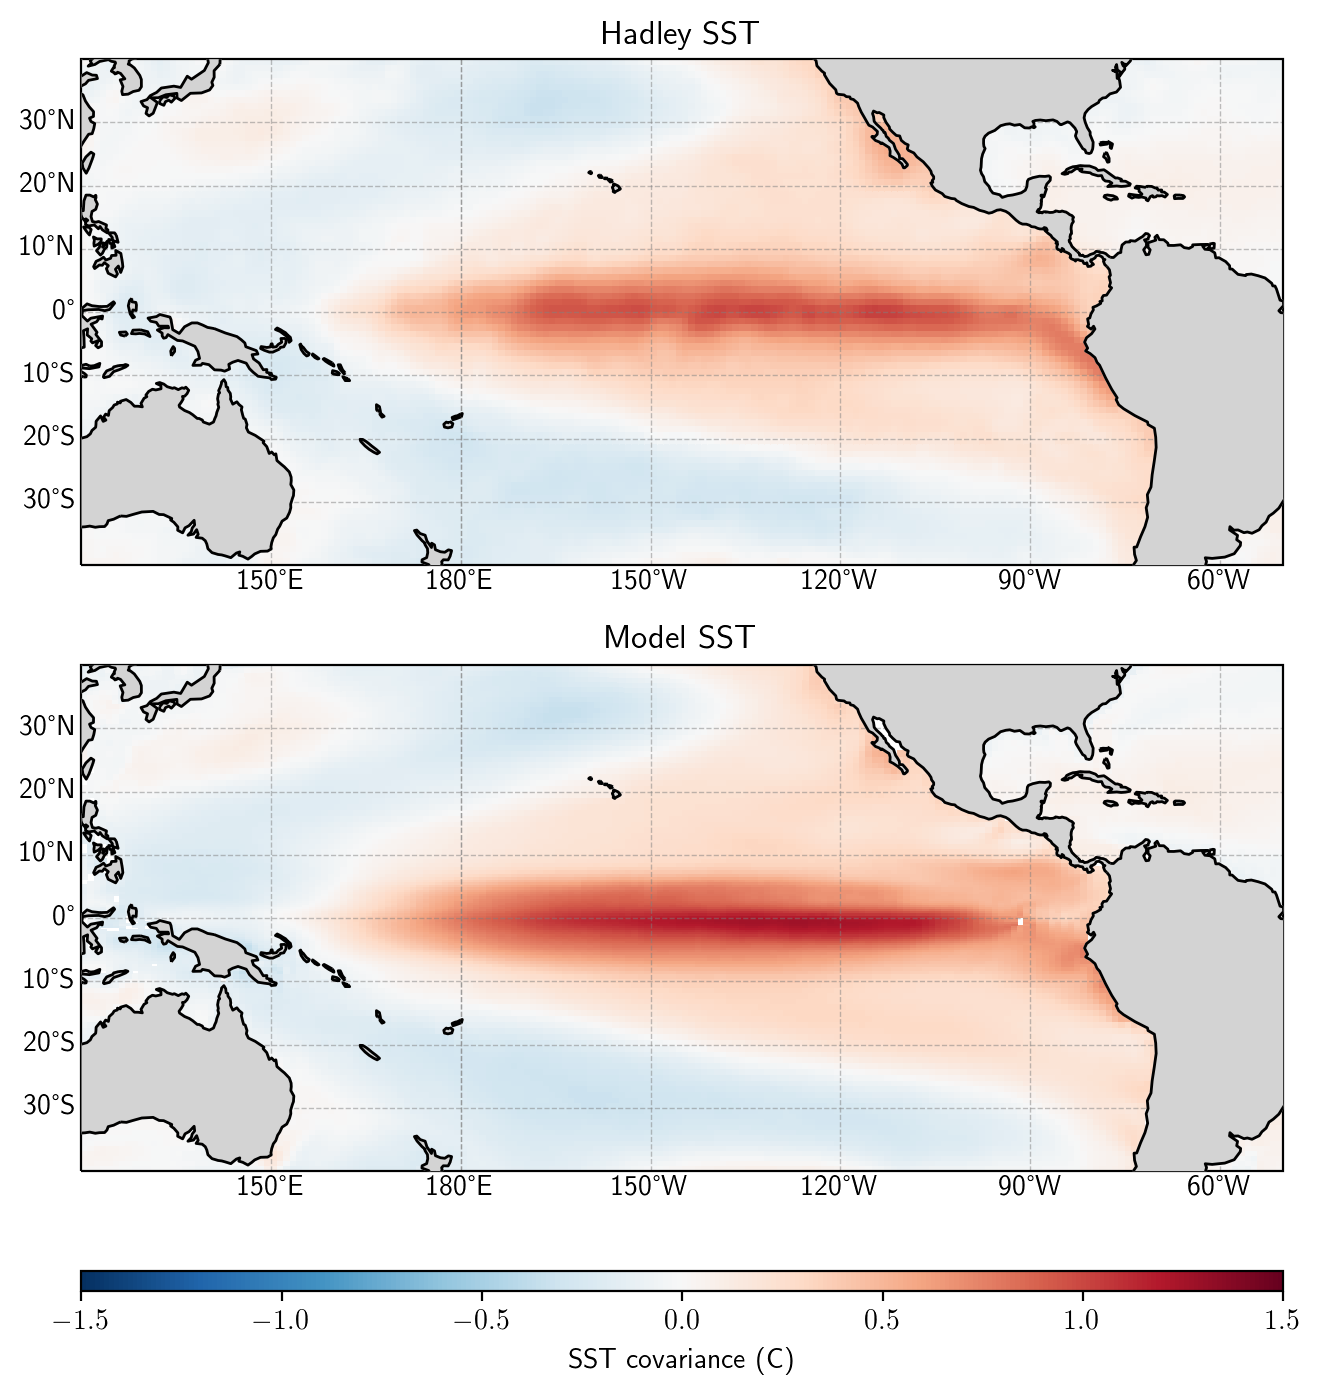
\includegraphics[scale=0.75] {scripts/cov-hadley/covariance_maps_hadley_model.png}
	\caption{Covariance between winter ONI index and Hadley (top) and simulated (bottom) yearly SST anomalies.}
	\label{fig:cov-sst}
\end{figure}

\subsection{Observed and simulated sea-surface chlorophyll}

In order to validate the biogeochemical response of the NEMO-Pisces model, satellite based observations of ocean colour \citep{sathyendranathOceanColourTimeSeries2019} have been used. The OceanColour-CCI V5 dataset provides monthly chlorophyl-a with a horizontal resolution of $1/24$\degree . First, data were Pacific-centerred and regridded to a one degree resolution. This was done by computing the weighted mean over $24 \times 24$ boxes, the weights being provided by the cosine of latitude. Coarse resolution grid cells that contained more than $1/3$ of missing data were considered as missing. Then, a monthly climatology was computed over the 1998-2020 period and removed from the observations. Finally, the covariance between these monthly anomalies and the monthly ONI index was computed between 1997-09 and 2018-12.  In a similar way, the covariance between the ONI index and the simulated surface chlorophyll was computed over the same period.\\

Covariance maps between the surface chlorophyll and the monthly ONI index are shown in figure \ref{fig:chl-cov}. The observations (upper panel) and the model (lower panel) show very similar covariance pattern, with a decrease in chlorophyll concentration in the tropical Pacific ocean, which is consistent with a reduction of the equatorial upwelling induced by the reduction and eventually reversal of the trade winds (\warn{REF}). However, the model overestimates the chlorophyll response to ENSO variability compared with observational based estimates. Note that the covariance for the simulated chlorophyll has also been computed over the entire simulated period (1958-2018), with no significant changes in the resulting pattern (not shown). \\

\begin{figure}[h!]
	\centering
	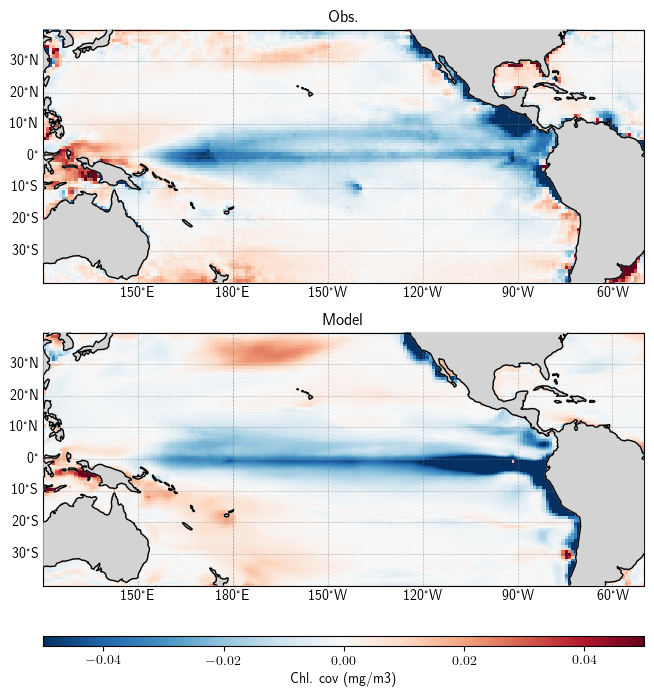
\includegraphics[scale=0.75] {scripts/chl-sat/compare_covariance_chl.png}
	\caption{Covariance between the monthly ONI index and the monthly surface chlorophyll anomalies, computed between 1997-09 and 20018-12.}
	\label{fig:chl-cov}
\end{figure}
\section{Biological response to ENSO variability}

In order to investigate the response of fish biomass to ENSO variability, the methodology described in section \ref{sec:pisces} has been applied on the vertically integrated fish biomass density ($J.m^{-2}$).
For the sake of simplicity, the focus will be laid on three size classes: 2 cm, representing small fishes, 20cm, representing intermediate sizes, and 90 cm, representing large individuals. These sizes are also
representative of the sizes of tuna target species within the region.
\warn{ref!!!}.  \\ 

The covariance maps are shown in figure \ref{fig:cov-ape} for the three sizes and the three simulated generic communities. 

Small epipelagics show negative anomalies shows negative anomalies at around 5N and 5S, and shows slightly positive anomalies 
near the equator. Intermediate epipelagics show positive anomalies in the central Pacific and negative ones in the west.
The pattern for large epipelagics is similar to that of intermediate sizes, although the positive anomalies are weaker and shifted westward.\\

The covavariance maps for the small migrants shows anomalies in the western part of the domain and along the coast of South America. Anomalies are also negative in the west for intermediate migrants but with negative anomalies in the central Pacific and in the east. The anomalies for large migrant fishes show an alternance of positive and negative anomalies along the equator. \\

Small mesopelagics shows positive anomalies in the central Pacific, and negative anomalies in the west.  
This pattern is very similar to that of intermediate epipelagics, although the magnitudes are different and are westward shifted. Intermediate and large mesopelagics show positive anomalies in the western part of the basin. \\ 

\begin{figure}[h!]
    \centering
    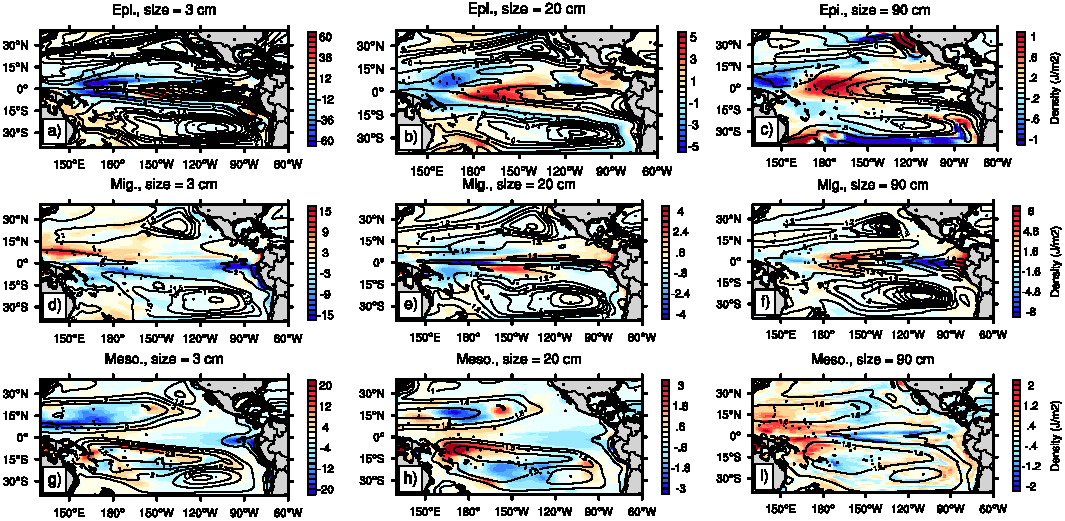
\includegraphics[width=\textwidth] {figs/debugged_corr_mask_covariance_maps_OOPE.pdf}
    \caption{Covariance between winter ONI index and \ap\ vertically integrated fish biomass density ($J.m^{-2}$). Mean biomass density is shown in black contour lines (log scale).}
    \label{fig:cov-ape}
\end{figure}

\subsection{Transient biological response to \nino}

\begin{figure}[h!]
    \centering
    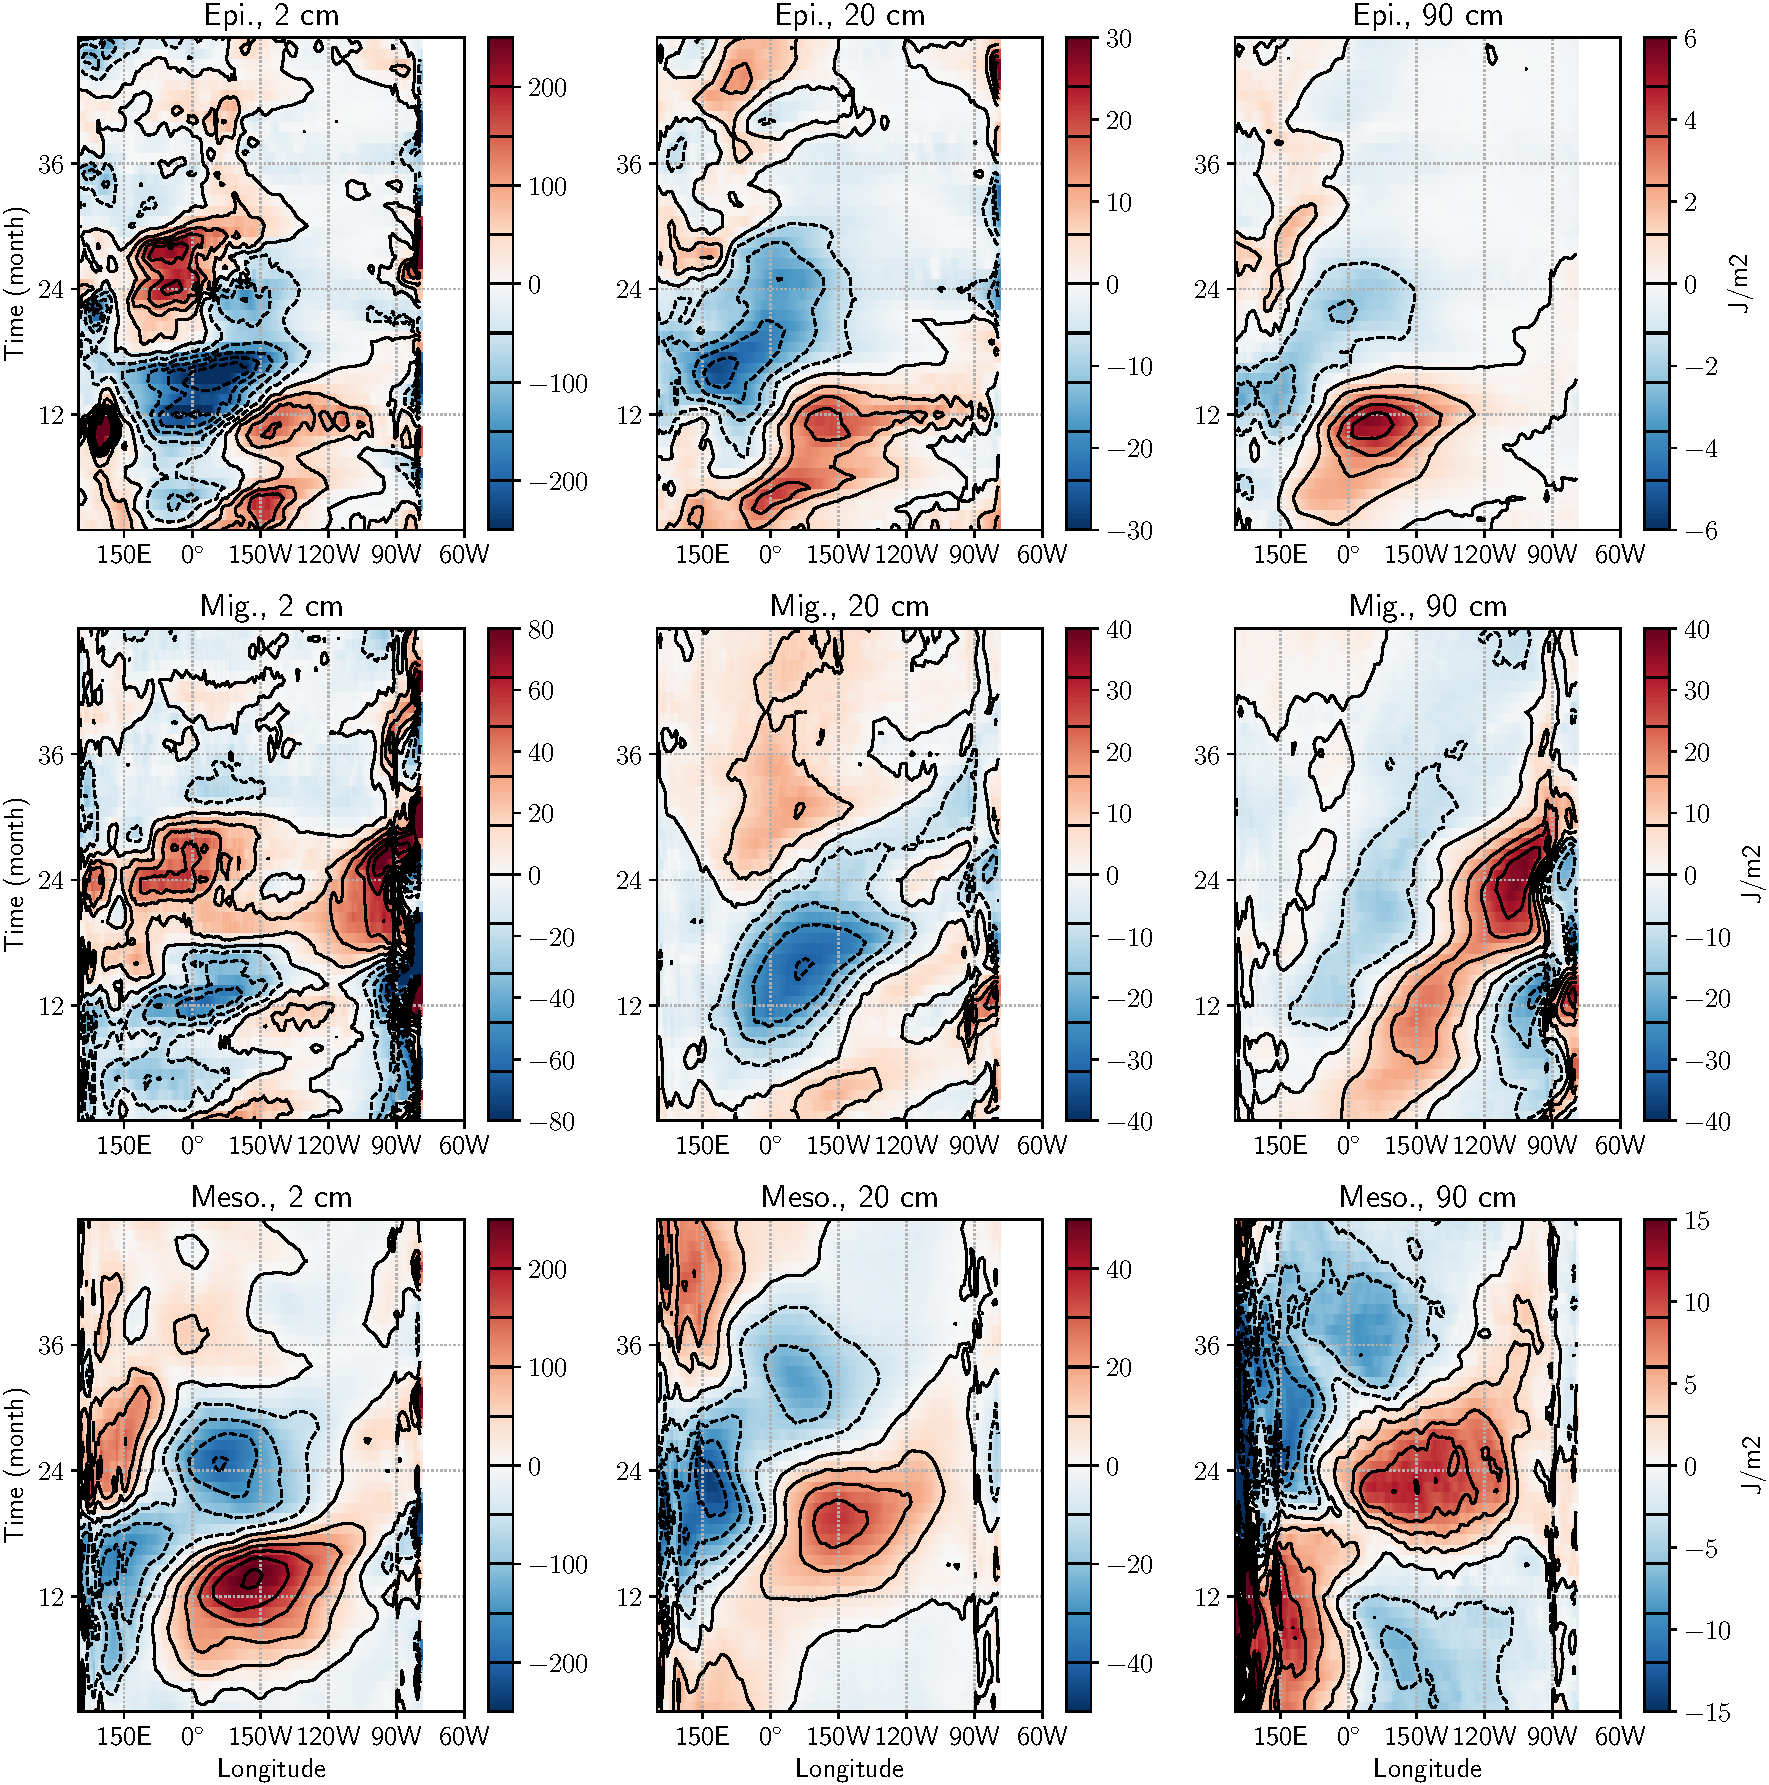
\includegraphics[scale=0.5] {corr_mask_hovmoller_composites_OOPE}
    \caption{Composites of \hov\ diagram composite of fish biomass density ($J.m^{-2}$) along the equatorial Pacific ocean.}
    \label{fig:hov-oope}
\end{figure}

\clearpage

\section{Discussions}

In the present paper, we analysed the response of fish biomass to changes in the physical and biogeochemical ocean in response to ENSO variability. The Apecosm model was forced by the outputs of the NEMO/Pisces physical and biogeochemical model, with no retroaction of the former on the latter. One question that arises is whether the response of fish biomass and ocean biogeochemistry to ENSO variability would be the same in a two-way coupled simulation. 	Such coupling, which has already been used in \cite{aumontEvaluatingPotentialImpacts2018} to analyse the impacts of the diurnal vertical migration on ocean biogeochemistry, could be used to determine whether the inclusion of fish biomass modifies the response of ocean biogeochemistry to ENSO. And whether the coupling attenuates or strengthens the response of fish biomass. Improve the text.
 
The study relies on a global simulation at a relatively coarse horizontal resolution (around 1°), which is insufficient to explicitly represents the mesoscale features of the California Current System \citep{capetMesoscaleSubmesoscaleTransition2008} and of the Peru-Chile current system \citep{colasHeatBalanceEddies2012}. This may lead to a misrepresentation of temperature and biogeochemical variables in the upwelling systems, which will ultimately propagates to the higher trophic levels. Guiet et al. (in prep) have used Apecosm on a regional configuration of the California Current Ecosystem. They show that small sizes emerge from the coast, where they are trapped in mesoscale features where plankton biomass is abundant, and are advected westward while they grow.

In this study, the transient response of marine ecosystems has been investigated from covariance analysis using a single El Nino index. This methodology assumes that ENSO variability is linear, i.e. that positive ENSO phases (El Nino) are opposite to negative ENSO phases (La Nina), which is not the case \citep{larkinENSOWarmNino2002}. Furthermore, no distinction has been made between the Eastern Pacific Nino (EPN) and the Central Pacific Nino (CPN) events, which have different physical and biogeochemical signatures and causes. For instance, \cite{gierachBiologicalResponse19972012} have shown, using satellite observations and adjoint passive tracer simulations, that EPN causes a reduction chlorophyll-a in the Eastern Pacific, mainly due to weaker trade winds, reduced upwelling and vertical mixing, while CPN reduces chlorophyll-a in the Central Pacific, mainly through a stronger eastward advection of nutrient-depleted waters from the Western Pacific. These different type of El Nino events may therefore have different impacts on fish biomass.

In the present study, changes in fish biomass in relation with ENSO variability are potentially driven by changes in temperature, oxygen or plankton concentration. In order to distinguish these different effects, sensitivity simulations can be run, for instance by using a temperature climatology instead of an interannual one. 

• Coupling NEMO-Pisces and impacts?  % done
• Regional simulations to better represents physical processes? %done
• Focus species (tuna), more suited for tropical pacific
• ENSO impacts in the other regions (cf. Racault)  
• Separation of CP/EP Ninos  % done
• Different communitities
• Sensitivity experiments (climPlk, climTemp)
• Impacts of other modes of variabilities (PDO, NAO, AR).

\warn{\cite{racaultImpactNinoVariability2017} for impact on plankton}



\listoffigures
\listoftables

\clearpage

\bibliography{ApecosmBib2}

\end{document}
